% Overview:
%   MALVA TeX subfile for the project.
%   Each subfile MUST start with the following line
%		\documentclass[../main.tex]{subfiles}

\documentclass[../main.tex]{subfiles}

\begin{document}

\subsection{MALVA}
\label{malva}

Il secondo framework che viene presentato è MALVA \cite{bernardini2019malva}. I metodi standard \textit{reference based} ed \textit{alignment free} si concentrano su SNP isolati e bi-allelici, fornendo un supporto limitato per SNP multi-allelici e per gli indel, inserimenti ed eliminazioni di nucleotidi. MALVA si propone come un nuovo metodo \textit{mapping free} per genotipizzare un individuo da un campione di read, permettendo di individuare SNP multi-allelici (cioè varianti in cui è noto più di un allele alternato) e indel, brevi e lunghi, anche in regioni genomiche ad alta densità, e di gestire efficacemente un grande numero di varianti. 

MALVA è un metodo basato su \textit{word}: a ciascun allele, di ciascuna variante nota, viene assegnata una firma (\textit{signature}) sotto forma di un insieme di \textit{k}-mer, che consente di modellare in modo efficiente SNP, indel e varianti: si effettua la chiamata dei genotipi in base alla frequenza delle \textit{signature} nelle read in input. Inoltre, prendendo come base la formula di Bayes, l'algoritmo propone una nuova regola per genotipizzare varianti multi-alleliche.

\cite{bernardini2019malva} dichiarano che è un tool rapido, leggero e privo di allineamento per genotipizzare varianti note e richiede un ordine di grandezza di tempo in meno per genotipizzare un donatore rispetto agli strumenti basati sull'allineamento, fornendo una precisione simile. Anche se le varianti multi-alleliche sono più difficili da genotipizzare rispetto a quelle bi-alleliche, riesce ad ottenere alta precisione. In merito a indel, MALVA fornisce risultati migliori rispetto agli strumenti più ampiamente adottati per rilevarli. 


\subsubsection{Definizioni e Struttura Dati di MALVA}

Il framework prende in input il genoma di riferimento, una lista di varianti e un set di read e restituisce in output un file VCF contenente il genotipo più probabile per ogni variante. Le varianti sono codificate in un file VCF (Variant Calling Format): ogni riga del file definisce una variante e contiene le relative informazioni; le varianti considerate sono SNP e indel.

Prima di specificare il concetto di \textit{signature} di un allele che è alla base dell'algoritmo, riportiamo alcune brevi definizioni: data una variante \textit{v}, indichiamo POS(\textit{v}) la posizione di \textit{v} nel riferimento, REF(\textit{v}) l'allele di riferimento, ALT(\textit{v}) l'elenco degli alleli alternati, FREQ(\textit{v}) l'elenco delle frequenze degli alleli, GTD(\textit{v}) i dati genotipici e, dato un allele \textit{a} (di riferimento o alternato) di \textit{v}, SEQ(\textit{a}) la sequenza di nucleotidi o stringa che rappresenta \textit{a}.

\theoremstyle{definition}
\begin{definition} 

Sia \textit{G} l'insieme di tutti i genomi codificati da un file VCF V e sia \textit{k} un valore dispari positivo. Sia \textit{v} una variante in V, \textit{a} un allele di \textit{v} e $\textit{G}^{a} \subseteq \textit{G}$, l'insieme dei genomi che contengono \textit{a}. Se SEQ(\textit{a}) è più lunga di \textit{k} si definisce come \textit{signature} di \textit{a} l'insieme di tutte le sottostringhe di lunghezza \textit{k} di SEQ(\textit{a}). In caso contrario, se SEQ(\textit{a}) ha lunghezza inferiore a \textit{k}, si definisce come \textit{signature} di \textit{a} nel genoma \textit{g} in $\textit{G}^{a}$ $\{ \textit{x}SEQ(\textit{a})\textit{y} \} $ se: (1) $\textit{x}SEQ(\textit{a})\textit{y}$ è un \textit{k}-mer, (2) $|\textit{x}| = \lfloor \frac{k-|SEQ(\textit{a})|}{2} \rfloor$, (3) $|\textit{y}| = \lceil \frac{k-|SEQ(\textit{a})|}{2} \rceil$, (4) \textit{x} è un suffisso della sequenza che precede \textit{a} in \textit{g}, (5) \textit{y} è un prefisso della sequenza che segue \textit{a} in \textit{g}.

\end{definition}

\noindent
Intuitivamente, la firma dell'allele \textit{a} di una variante \textit{v} è il \textit{k}-mer centrato in \textit{a} (che quindi contiene \textit{a} in posizione centrale) in qualche genoma \textit{g} che include \textit{a}. A seconda dei genomi codificati dal file VCF, in particolare, se sono note altre varianti a meno di \textit{k} basi di distanza dall'allele, esso potrebbe avere più firme: la definizione quindi ammette la presenza di alleli di più varianti in una sola firma, consentendo a MALVA di gestire varianti che sono vicine. Inoltre, se la stringa di basi che rappresenta l'allele è più lunga di \textit{k}, non esiste un \textit{k}-mer che può essere centrato in \textit{a}: in questo caso, la firma è l'insieme delle sue sottostringhe di lunghezza \textit{k}. L'insieme di tutte le possibili firme di un allele \textit{a} viene chiamato SIGN(\textit{a}) e rappresenta tutte le regioni del genoma in cui l'allele appare nei genomi codificati dal file VCF di input. Nella Figura \ref{fig:malvaSign} si può vedere un esempio di calcolo di signature.

 \begin{figure}[h!]
	\centering
  	\captionsetup{justification=justified}
 	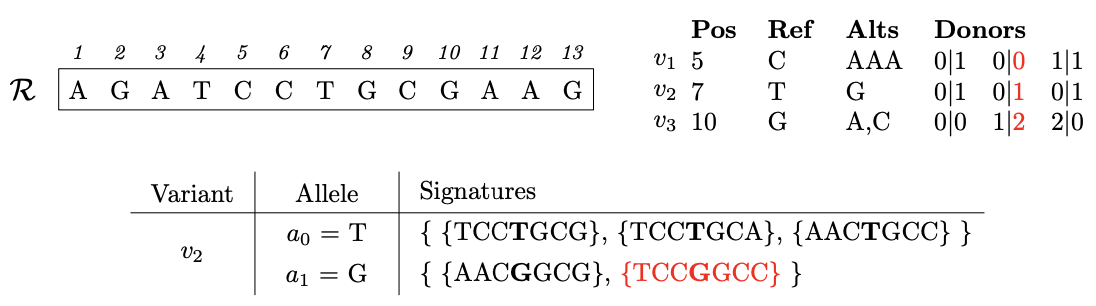
\includegraphics[scale=.65]{images/malva-sign.png}
  	\caption{Firme degli alleli della variante $v_{2}$. \textit{\textbf{R}} è la sequenza di riferimento, la tabella a destra contiene le informazioni associate nel file VCF, che rappresentano 3 varianti: un indel ($v_{1}$), un SNP bi-allelico ($v_{2}$) e un SNP multi-allelico ($v_{3}$). Le ultime colonne del file VCF riportano le informazioni sul genotipo di 3 individui. La tabella in basso riporta le firme di ciascun allele della variante $v_{2}$. Ci sono solo 5 firme sebbene 6 aplotipi siano codificati dal file VCF poiché il secondo aplotipo del primo e del terzo individuo sono gli stessi.}
  	\label{fig:malvaSign}
\end{figure}


Nel corso del procedimento per determinare il genotipo delle varianti, le firme vengono salvate in 3 set: REFSIG, che contiene le firme di alleli di riferimento, ALTSIG, che contiene firme di alleli alternati, e REPCTX che memorizza il contesto attorno ad alcune firme di alleli alternati che compaiono identiche anche in altre regioni del genoma. ALTSIG è costruito con un Bloom Filter ed una singola funzione di hash\footnote{\ Nota \vref{nota:OHBF}.}, in quanto, una volta che tutte le firme di tutti gli alleli alternati sono state aggiunte ad ALTSIG, il set viene utilizzato solo per verificare se alcuni \textit{k}-mer fanno parte di una firma. Una volta costruito questo set, in base al numero di 1 nel Bloom Filter (ovvero al numero di \textit{k}-mer in ALTSIG) viene associato un array di interi in cui verranno salvati i pesi (contatori) dei \textit{k}-mer; di fatto, l'uso di una singola funzione hash consente di archiviare i pesi in modo efficiente per ogni \textit{k}-mer. Allo stesso modo, anche REPCTX viene implementato tramite un Bloom Filter ad una singola funzione hash. Viceversa, REFSIG è implementato come una semplice tabella hash, poiché il numero di elementi che memorizza è generalmente inferiore al numero di elementi memorizzati in ALTSIG. 


\subsubsection{Algoritmo di MALVA}

L'algoritmo utilizza la definizione di \textit{signature} di un allele e la sua frequenza per rilevare la sua presenza in un individuo (nelle read) senza effettuare l'allineamento delle read sul genoma di riferimento e chiamare il genotipo. Esso funziona supponendo che, dato un campione di read da un genoma, se un allele è incluso nel genoma, almeno una delle sue firme deve esistere come sottostringa in read multiple. 

Nella sottostante Figura \ref{fig:malva} è riportata graficamente la pipeline di MALVA. In seguito saranno esaminati in dettaglio le quattro fasi su cui si basa il metodo principale.

 \begin{figure}[h!]
	\centering
  	\captionsetup{justification=centering}
 	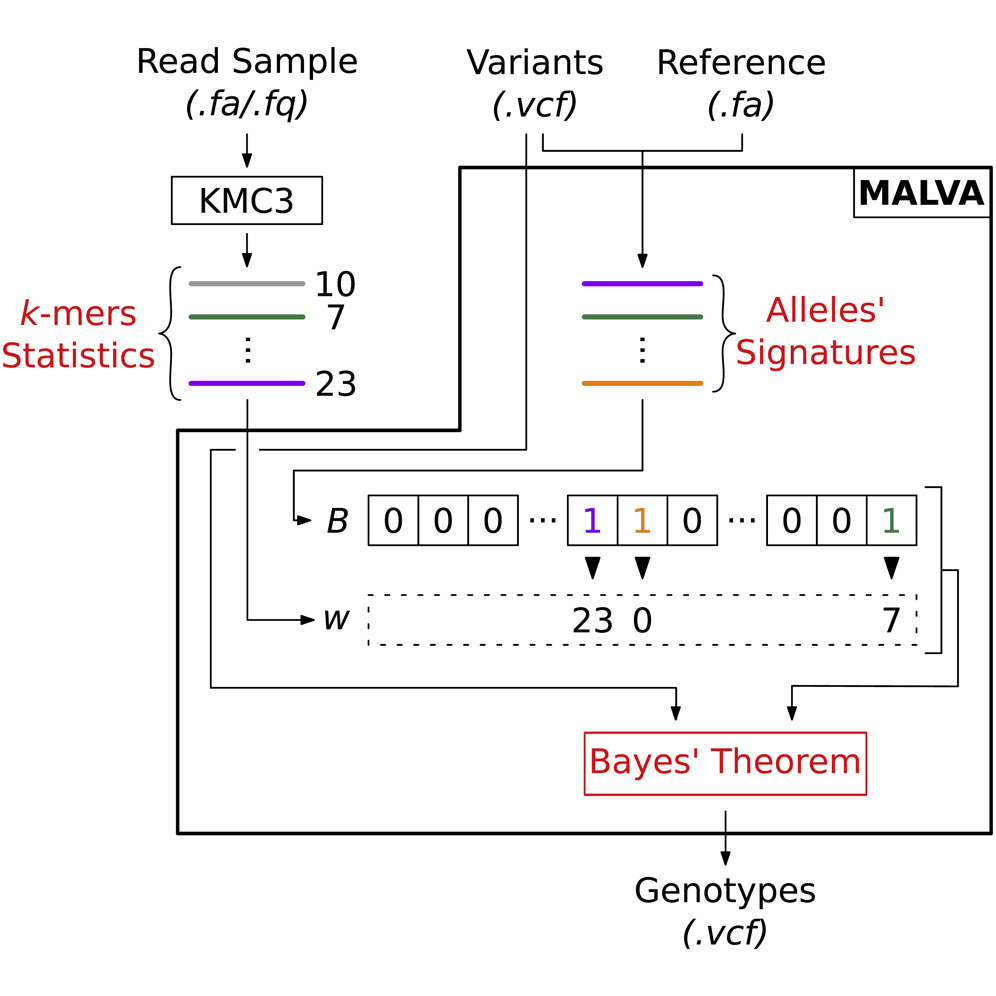
\includegraphics[scale=.85]{images/malva-pipeline.jpg}
  	\caption{Pipeline, MALVA.}
  	\label{fig:malva}
\end{figure}

\noindent
\textbf{Step 1} Si calcola l'insieme delle firme di lunghezza \textit{${k}_{s}$} di tutti gli alleli alternati di tutte le varianti nel file VCF che vengono memorizzate in ALTSIG. Le firme degli alleli di riferimento vengono invece calcolate e memorizzate in REFSIG. Quindi, vengono memorizzati due pesi per ogni \textit{${k}_{s}$}-mer \textit{t} di una firma: \textit{$w_{t}^{A}$} rappresenta il numero di occorrenze di \textit{t} nella \textit{signature} di un allele alternato e \textit{$w_{t}^{R}$} nella \textit{signature} di un allele di riferimento. Nel costruire le firme di un allele MALVA controlla tutti gli alleli delle varianti nel raggio di $\lfloor \frac{ {{{k}_{s}} }}{2}  \rfloor$ e usando il file VCF ricostruisce le sequenze in base alle informazioni sul genotipo. 

\paragraph{Step 2} Successivamente MALVA effettua il rilevamento delle \textit{signature} ripetute: per piccoli valori di  \textit{${k}_{s}$} la probabilità che i  \textit{${k}_{s}$}-mer che compongono una firma compaiano in altre regioni del genoma è alta. Poiché si sfrutteranno le firme degli alleli di ciascuna variante per chiamare i genotipi, la presenza di regioni conservate del genoma di riferimento identiche a una firma potrebbero portare il framework a genotipizzare erroneamente alcune varianti. Si utilizza perciò il contesto attorno all'allele per distinguere le firme da tali regioni. Se un  \textit{${k}_{s}$}-mer di una firma di un allele alternato appare in qualche parte nel genoma di riferimento, MALVA estrae il contesto di lunghezza  \textit{${k}_{c}$} della regione del genoma di riferimento attorno a tale \textit{${k}_{s}$}-mer (con  \textit{${k}_{c}$} $>$ \textit{${k}_{s}$}) e raccoglie tali \textit{${k}_{c}$}-mer in REPCTX. In questo modo, rileva e memorizza tutti i \textit{${k}_{c}$}-mer della sequenza di riferimento il cui \textit{${k}_{s}$}-mer centrale è incluso in alcune \textit{signature} di alleli alternati. 

\paragraph{Step 3} MALVA usa KMC3 \cite{Kokot2017KMC3} per estrarre i \textit{${k}_{c}$}-mer delle read in maniera efficiente ed effettuare il conteggio delle loro occorrenze: KMC3 è un algoritmo molto efficacie per eseguire il \textit{k-mer counting}. Per ogni \textit{${k}_{c}$}-mer  \textit{${t}_{c}$} che appare \textit{w} volte nel campione, viene quindi estratto il \textit{${k}_{s}$}-mer  \textit{${t}_{s}$} centrale. Se \textit{${t}_{s}$} è in REFSIG, ovvero è la firma dell'allele di riferimento di una variante, \textit{$w_{{t}_{s}}^{R}$} è aumentato di \textit{w}. Se \textit{${t}_{c}$} non è in REPCTX e \textit{${t}_{s}$} è in ALTSIG, \textit{$w_{{t}_{s}}^{A}$} viene aumentato di \textit{w}. Altrimenti, se \textit{${t}_{c}$} è in REPCTX, \textit{$w_{{t}_{s}}^{A}$} non viene aggiornato, poiché sebbene il suo \textit{${k}_{s}$}-mer centrale sia uguale ad alcuni \textit{signature} \textit{${k}_{s}$}-mer di allele alternato, è indistinguibile da un'altra regione del genoma che non copre la variante. Notiamo che quando \textit{$w_{{t}_{s}}^{A}$} non viene aggiornato, potrebbe esserci la possibilità di non contare una variante del donatore e riportare un falso negativo: si preferisce evitare bias dovuti ai \textit{${k}_{c}$}-mer nelle regioni conservate del genoma di riferimento e, ogni volta che sorgono ambiguità, non contare l'allele alternato; per grandi valori di  \textit{${k}_{c}$} questo, tuttavia, accade raramente. 

\paragraph{Step 4} Infine MALVA utilizza i pesi delle \textit{signature} calcolati nella fase precedente e le informazioni sugli alleli memorizzate nel file VCF in input per determinare il genotipo di ciascuna variante. Vengono estesi gli approcci proposti in letteratura per le varianti bi-alleliche, in particolare quello introdotto in LAVA \cite{shajii2016lava}, alle varianti multi-alleliche, poiché è necessario calcolare la probabilità dei vari possibili genotipi. Data \textit{v} una variante con (\textit{n} - 1) alleli alternati, il numero di possibili genotipi distinti è $\binom{n}{2} + n = \dfrac{n(n+1)}{2}$, rispettivamente un genotipo di riferimento omozigote, $\binom{n}{2}$ genotipi eterozigoti e (\textit{n} - 1) genotipi alternati omozigoti. MALVA calcola la probabilità di ciascun genotipo utilizzando il teorema di Bayes e il teorema della probabilità assoluta. Viene calcolata la probabilità a priori di ogni genotipo e la probabilità condizionata della coverage osservata dato il genotipo considerato: per computare queste probabilità vengono nuovamente usate le \textit{signature} e i pesi calcolati nelle fasi precedenti. Dopo aver determinato la probabilità di ciascun genotipo, MALVA restituisce in output come genotipo predetto quello con la più alta probabilità.


\end{document}